% Copyright (c) 2005-2008 Center for Urban Simulation and Policy Analysis,
% University of Washington.  Permission is granted to copy, distribute and/or
% modify this document under the terms of the GNU Free Documentation License,
% Version 1.2 or any later version published by the Free Software Foundation;
% with no Invariant Sections, no Front-Cover Texts, and no Back-Cover Texts.
% A copy of the license is included in the section entitled "GNU Free
% Documentation License".

\chapter{UrbanSim Structure and Specification of Model Components}
\label{chapter:models}

UrbanSim takes several key inputs as exogenous.  Two of these are
from external model systems: a macroeconomic model to predict
future macroeconomic conditions such as population and employment
by sector, and a travel demand model system to predict travel
conditions such as congested times and composite utilities of
travel between each interchange.  The latter is loosely coupled to
UrbanSim, with land use predictions input to the external travel
models, and travel conditions input to subsequent annual
iterations of the UrbanSim land use model system.

\begin{figure}
\begin{center}
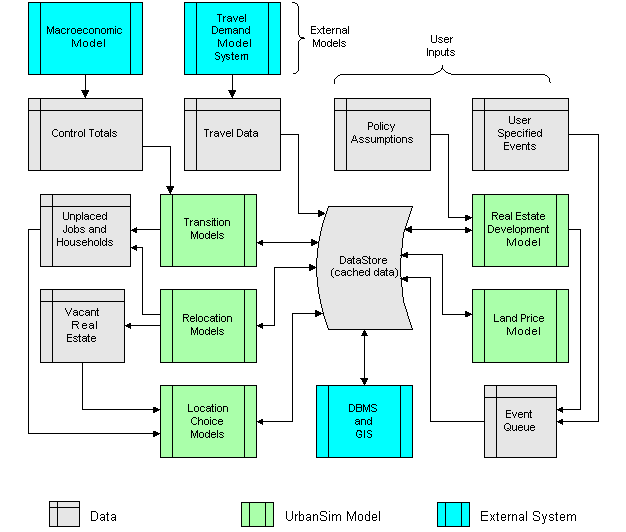
\includegraphics[width=6.5in]{images/flownew.png}
\caption{UrbanSim Model Structure} \label{figure:USStruct}
\end{center}
\end{figure}

UrbanSim operates on an annual scheduling of key model components,
and data flow is as shown in Figure \ref{figure:USStruct}.  The data
store contains the current state of all objects in the system,
with archiving as needed by individual model components, or as
requested by the model user into ASCII extracts from the model.
Each of the key model components are described in the following
sections.  The mathematical structure of the underlying procedures
in the model are virtually identical for the household and
employment aspects of the model system, so for brevity the
household equations are omitted from the presentation below.

The model system reads exogenous inputs not only from external
macroeconomic and travel demand models, but also from user input.
These user inputs include assumptions reflecting land use policies
that regulate real estate development, and any user-specified
events that describe scheduled events representing changes in
employment, real estate development or land policy the user
intends to apply to the model in a simulation year beyond the
initial, or base year.

The main model components, in the order of their execution, are
the economic and demographic transition models, the household and
employment mobility models, the accessibility model, the household
and employment location choice models, the real estate development
model, and the land price model.  An export model writes
simulation results in user-specified forms to output files for
further analysis or processing, such as by travel demand models or
by GIS.

Locations in the model are based on a grid with a resolution of
150 by 150 meters per grid cell.  Cells are cross-referenced to
Traffic Analysis Zone for indexing travel model outputs, and to
city, county, and other geographic overlays for indexing land use
policies that apply to specific jurisdictions or overlays.

\section{Economic Transition Model}
Employment is classified by the user into employment sectors based
on aggregations of Standard Industrial Classification codes.
Typically 10 to 20 sectors are defined based on the local economic
structure. Aggregate annual forecasts of economic activity and sectoral
employment are exogenous to UrbanSim, and are used as inputs to
the model. These forecasts may be obtained from state economic
forecasts or from commercial or in-house sources.

The Economic Transition Model compares these exogenous
forecasts of aggregate employment by sector with the
UrbanSim employment data, computes the sectoral growth or
decline from the preceding year, and either queues jobs to
be placed in the employment location choice model for
sectors that experience growth, or removes jobs from the
database in sectors that are declining.  In cases of sectors
with employment growth, new jobs are sampled from existing
jobs of the same sector with location identifier (grid_id)
set to uplaced.  While in cases of sectors with employment
loss, jobs will be randomly picked to be removed with
probability proportional to the number of jobs in the
sector.  The jobs that are removed vacate the space they
were occupying, and this space adds to the pool of vacant
space and becomes available for other jobs to occupy in the
employment location choice model.  This procedure keeps the
accounting of land, structures, and occupants up to date.

New jobs are not immediately assigned a location.  Instead,
new jobs are added to the database and assigned a null
location, to be allotted by the Employment Location Choice
Model. The model proceeds as follows.

Calculate the number of jobs to be added or removed (a
scalar).
\begin{equation}
\Delta J_{st} = C_{st} - |J_{s(t-1)}|,
\end{equation}
where:
\begin{center}
\begin{tabular}{c p{5.5in}}
$\Delta J_{st}$ & is the change from year $t-1$ to $t$ in number of jobs in sector $s$,\\
$C_{st}$ & is the exogenous total employment in sector $s$ in year $t$,\\
$J_{s(t-1)}$ & is the set of all jobs in sector $s$ in year $t-1$,\\
$|.|$ returns the number of elements in (cardinality of) the set.\\
\end{tabular}
\end{center}

The set of all jobs at year $t$ is defined by one of three cases.
Either it is the union of the previous year's jobs and some newly
created jobs or the difference between the previous year's jobs
and some number of jobs to remove.

\begin{equation}
J_{st} =
    \begin{cases}
        J_{s(t-1)} \cup F_{st}, &\text{if $\Delta J_{st} > 0$}, \\
        J_{s(t-1)} &\text{if $\Delta J_{st} = 0$},\\
        J_{s(t-1)} - F_{st}, &\text{if $\Delta J_{st} < 0$},
    \end{cases}
\end{equation}
where:
\begin{center}
\begin{tabular}{c p{5.5in}}
$F_{st}$ & is the set of jobs in flux in sector $s$ in year $t$, \\
\end{tabular}
\end{center}

The set of jobs in flux $F_{st}$ is a set of jobs being
added to or removed from sector $s$ in year $t$. It is
uniformly sampled from jobs set $J_{s(t-1)}$.

\begin{equation}
F_{st} = \{\, j \in J_{s(t-1)} \,\},
\end{equation}
and
\begin{equation}
| F_{st} | = | \Delta J_{st} |.
\end{equation}
%
The cardinality of flux jobs is equal to the absolute value of the
change in number of jobs.

If we are adding new jobs, then jobs in $F_{st}$ will be
unplaced from their current location by changing their
location attribute to a pre-defined constant for unplaced.

%% \begin{equation}
%% F_{st} = \{\, L_j = U, j \in F_{st} \,\}, &\text{if $\Delta J_{st} > 0$}, \\
%% \end{equation}
%% where:
%% \begin{center}
%% \begin{tabular}{c p{5.5in}}
%% $L_j$ & is the location of job $j$, \\
%% $U$ & is the pre-defined constant indicating a location has not been assigned. \\
%% \end{tabular}
%% \end{center}

This set of jobs will be added to the set of unplaced jobs
in the previous year and will be allotted to locations by
the Employment Location Choice Model later.
\begin{equation}
J^U_{st} = \begin{cases}
        J^U_{s(t-1)} \cup F_{st}, & \Delta J_{st} > 0,\\
        J^U_{s(t-1)}, & \text{otherwise},\\
    \end{cases}
\end{equation}
where:
\begin{center}
\begin{tabular}{c p{5.5in}}
$J^U_{st}$ & is the set of jobs that do not have a location match at time $t$.\\
\end{tabular}
\end{center}

If we are removing jobs, then those jobs in $F_{st}$ will be
removed from jobs set $J_{s(t-1)}$, and the space they
occupied will be released and become available to unplaced
jobs for location choice.

\begin{equation}
S_{lt} = \begin{cases}
        S_{l(t-1)} + s^l_j \mid j \in F_{st}, (j, l) \in M^l_{j(t-1)},  \Delta J_{st} < 0,\\
        S_{l(t-1)}, & \text{otherwise},\\
    \end{cases}
M^l_{jt} = M^l_{j(t-1)} - \{\, (j, l) | j \in F_{st}, (j, l) \in M^l_{j(t-1)} \}\, \Delta J_{st} < 0, \\
\end{equation}
where:
\begin{center}
\begin{tabular}{c p{5.5in}}
$S_{lt}$ & is the available space for location (gridcell) $l$ at time $t$,\\
$s^l_j$ & is the space job $j$ occupies at location $l$, \\
$M^l_{j(t-1)}$ is the pair of job/location matching job $j$ to location $l$ at time $t-1$. \\
\end{tabular}
\end{center}

So far we assume the space a job takes up depends on space utilization ratio of its location $r_l$.
\begin{equation}
s^l_j = r_l
\end{equation}

\section{Demographic Transition Model}

The Demographic Transition Model accounts for changes in the
distribution of households by type over time, using an algorithm
analogous to that used in the Economic Transition Model.  In
reality, these changes result from a complex set of social and
demographic changes that include aging, household formation,
divorce and household dissolution, mortality, birth of children,
migration into and from the region, changes in household size, and
changes in income, among others.  The data (and theory) required
to represent all of these components and their interactions
adequately are not readily available. Instead, the Demographic
Transition Model, like the Economic Transition Model described
above, uses external control totals of population and households
by type (the latter only if available) to provide a mechanism for
the user to approximate the net results of these changes. Analysis
by the user of local demographic trends may inform the
construction of control totals with distributions of household
size, age of head, and income.  If only total population is
provided in the control totals, the model assumes that the
distribution of households by type remains static.

As in the economic transition case, household births are added to
a list of movers that will be located by the Household Location
Choice Model.  Household deaths, on the other hand, are accounted
for by this model by removing those households from the housing
stock, and by properly accounting for the vacancies created by
their departure.  The demographic transition model is analogous in
form to the employment transition model described above.


\section{Employment Relocation Model}

Employment relocation and location choices are made by firms.
However, in the current version of UrbanSim, we use individual
jobs as the units of analysis.  This is equivalent to assuming
that businesses are making individual choices about the location
of each job, and are not constrained to moving an entire
establishment.

The Employment Relocation Model predicts the probability that jobs
of each type will move from their current location or stay during
a particular year. This is a transitional change that could
reflect job turnover by employees, layoffs, business relocations
or closures. Similar to the economic transition model when
handling job losses in declining sectors, the model assumes that
the hazard of moving is proportional to the spatial distribution
of jobs in the sector.  All placement of jobs is managed through
the employment location model.

As in the case of job losses predicted in the economic transition
component, the application of this model requires subtracting jobs
by sector from the buildings they currently occupy, and the
updating of the accounting to make this space available as vacant
space. These counts will be added to the unallocated new jobs by
sector calculated in the economic transition model. The
combination of new and moving jobs serve as a pool to be located
in the employment location choice model. Vacancy of nonresidential
space will be updated, making space available for allocation in
the employment location choice model.

Since it is possible that the relative attractiveness of
commercial space in other locations when compared with an
establishment's current location may influence its decision to
move, an alternative structure for the relocation model could use
the marginal choice in a nested logit model with a conditional
choice of location. In this way, the model would use information
about the relative utility of alternative locations compared to
the utility of the current location in predicting whether jobs
will move.  While this might be more theoretically appealing than
the specification given, it is generally not supported by the data
available for calibration. Instead, the relocation decision is
treated as an independent choice, and the probabilities estimated
by annual relocation rates directly observed over a recent period
for each sector.  The resulting form of the employment relocation
model is as follows.

$R_{st}$ is a set of jobs that are chosen to be moved based on $D(j,
t)$, a binary decision function based on Monte Carlo sampling
process using the annual relocation rate for sector $s$.
\begin{equation}
R_{st} = \{\, j \in J_{st} \mid D(j,t) \,\},
\end{equation}
where:
\begin{center}
\begin{tabular}{c p{5.5in}}
$R_{st}$ & is the set of jobs in sector $s$ at time $t$ that are
uprooted by the relocation model,\\
$D(j,t)$ & is a function based on Monte Carlo sampling process determining if job
$j$ will be moved at \mbox{time $t$}.\\
\end{tabular}
\end{center}

The jobs to be moved are now unplaced and added to the
unplaced jobs set, and the space they occupied will be released
and become available to unplaced jobs for location choice.

\begin{equation}
J^U_{st} = J^U_{st} \cup R_{st}
\end{equation}


\begin{equation}
S_{lt} = S_{l(t-1)} + s^l_j \mid j \in R_{st}, (j, l) \in M^l_{jt},\\
M^l_{jt} = M^l_{j(t-1)} - \{\, (j, l) | j \in R_{st}, (j, l) \in M^l_{jt} \}\, \Delta J_{st} < 0, \\
\end{equation}

\section{Household Relocation Model}

The Household Relocation Model is similar in form to the Employment
Relocation Model described above.  The same algorithm is used, but
with rates or coefficients applicable to each household type.  For
households, relocation probabilities are estimated from the Census
Current Population Survey, which provides a national database on
which annual relocation rates are computed by type of household.
This will reflect differential relocation rates for renters and
owners, and households at different life stages.

Application of the Household Relocation Model requires subtracting
mover households by type from the housing stock by cell, and
adding them to the pool of new households by type estimated in the
Demographic Transition Model. In the database, this is
accomplished by setting the location field for the moving
households to a null value.  The combination of new and moving
households serves as a population of households to be located by
the Household Location Choice Model. Housing vacancy is updated as
movers are subtracted, making the housing available for occupation
in the household location and housing type choice model.

\section{Real Estate Development Model}
\label{real-estate-development-model}

The real estate development model simulates the location choices of development
projects through the construction of new development.  Development projects of
different type choose locations where they will be developed.  The new model
looks basically like the other location choice models for households and for
jobs.  See Section~\ref{sec:development-project-lcm} for the technical details
of the implementation.

\section{Employment Location Choice Model}

In this model, we predict the probability that a job that is
either new (from the Economic Transition Model), or has moved
within the region (from the Employment Relocation Model), will be
located at a particular site.  The grid cells used as the basic
geographic unit of analysis in the current model implementation
contain variable quantities of space to be occupied by jobs. The
number of locations available for a job to locate within a grid
cell will depend mainly on the total square footage of
nonresidential floorspace in the cell, and on the density of the
use of space (square feet per employee). Given the possibility
that some jobs will be located in residential units, however,
housing as well as nonresidential floorspace must be considered in
job location.  We have defined a maximum rate of home-based
employment, determined using local data for a particular
metropolitan region, to identify the potential set of spaces
available for home-based employment. The set of job locations
available for placing a job, then, are the union of the spaces in
nonresidential floorspace and a subset of the residential units in
the cell. The model is specified as a multinomial logit model,
with separate equations estimated for each employment sector.

\begin{equation}
S_{blt} = s_{bl} / R_{bl}, for l \in L_t,
\end{equation}

where:
\begin{center}
\begin{tabular}{c p{5.5in}}
$S_{blt}$ & is the number of job space for building type $b$ at location $l$, \\
$s_{bl}$ & is a scalar representing the total nonresidential square footage of floorspace for building type $b$ in location $l$,\\
$r_{bl}$ & is a space utilization rate for building type $b$ in location $l$ (e.g. non-residential sqft per non-home-based employee, or housing units per home-based employee). \\
\end{tabular}
\end{center}

Since we process each building type in parallel, we can eliminate
subscript $b$ in the following equations.

For both the employment location and household location
models, we take the stock of available space as fixed in the
short run of the intra-year period of the simulation, and
assume that locators are price takers.  That is, a single
locating job or household does not have enough market power
to influence the transaction price, and must accept the
current market price as given.

The variables included in the employment location choice model are
drawn from the literature in urban economics.  We expect that
accessibility to population, particularly high-income population,
increases bids for retail and service businesses.  We also expect
that two forms of agglomeration economies influence location
choices: localization economies and inter-industry linkages.

Localization economies represent positive externalities associated
with locations that have other firms in the same industry nearby.
The basis for the attraction may be some combination of a shared
skilled labor pool, comparison shopping in the case of retail,
co-location at a site with highly desirable characteristics, or
other factors that cause the costs of production to decline as
greater concentration of businesses in the industry occurs.  The
classic example of localization economies is Silicon Valley.
Inter-industry linkages refer to agglomeration economies
associated with location at a site that has greater access to
businesses in strategically related, but different, industries.
Examples include manufacturers locating near concentrations of
suppliers in different industries, or distribution companies
locating where they can readily service retail outlets.

One complication in measuring localization economies and
inter-industry linkages is determining the relevant distance for
agglomeration economies to influence location choices.  At one
level, agglomeration economies are likely to affect business
location choices between states, or between metropolitan areas
within a state.  Within a single metropolitan area, we are
concerned more with agglomeration economies at a scale relevant to
the formation of employment centers.  The influence of proximity
to related employment may be measured using two scales: a regional
scale effect using zone-to-zone accessibilities from the travel
model, or highly localized accessibilities using queries of the
area immediately around the given grid cell.  Most of the spatial
queries used in the model are of the latter type, because the
regional accessibility variables tend to be very highly
correlated, and because agglomerations are expected to be very
localized.  Note that the use of radial queries surrounding grid
cells also avoids the problems of arbitrary zonal aggregations.

Age of buildings is included in the model to estimate the
influence of age depreciation of commercial buildings, with the
expectation that businesses prefer newer buildings and discount
their bids for older ones.  This reflects the deterioration of
older buildings, changing architecture, and preferences, as is the
case in residential housing.  There is the possibility that
significant renovation will make the actual year built less
relevant, and we would expect that this would dampen the
coefficient for age depreciation.  We do not at this point attempt
to model maintenance and renovation investments and the quality of
buildings.

Density, the inverse of lot size, is included in the location
choice model.  We expect businesses, like households, to reveal
different preferences for land based on their production functions
and the role of amenities such as green space and parking area. As
manufacturing production continues to shift to more horizontal,
land-intensive technology, we expect the discounting for density
to be relatively high.  Retail, with its concentration in shopping
strips and malls, still requires substantial surface land for
parking, and is likely to discount bids less for density.  We
expect service firms to discount for density the least, since in
the traditional urban economics models of bid-rent, service firms
generally outbid other firms for sites with higher accessibility,
land cost, and density.

We might expect that certain sectors, particularly retail, show
some preference for locations near a major highway, and are
willing to bid higher for those locations.  Distance to a highway
is measured in meters, using grid spatial queries.  We also test
for the residual influence of the classic monocentric model,
measured by travel time to the CBD, after controlling for
population access and agglomeration economies.  We expect that,
for most regions, the CBD accessibility influence will be
insignificant or the reverse of that in the traditional
monocentric model, after accounting for these other effects.

Calibration of the model is based on a geocoded establishment file
(matched to the parcel file to link employment by type to land use
by type).  A sample of geocoded jobs in each sector is used to
estimate the coefficients of the location choice model.  As with
the Household Location Choice Model, the application of the model
produces demand by each employment type for cell locations.

The employment location model processes each job in the mover
queue individually, and queries grid cells for alternative
locations to consider. These alternatives are sampled in
proportion to the capacity of the built space in the cell for
accommodating jobs, and the number of alternatives to consider may
be determined by the user.  Note that jobs may be located in
housing units, as is increasingly the case with home-based
employment through telecommuting and small independent home-based
businesses.  A logit model is applied to estimate the probability
that the current job will move to each of the alternative job
spaces under consideration.  Monte carlo simulation is used to
generate a decision to locate in a particular alternative, and
once this choice is made, the job is assigned to the cell, and the
respective quantities of vacant and used space in the cell are
updated.  If a preferred alternative for a job becomes unavailable
during a simulation run, having been chosen and occupied by a
previously locating job, the currently locating job is assigned
its next best available alternative.

The independent variables used in the employment location choice
model can be grouped into the categories of real estate
characteristics, regional accessibility, and urban-design scale
effects as shown below:

\begin{itemize}

\item Real Estate Characteristics \\
\emph{Prices} \\
\emph{Development type (land use mix, density)}

\item Regional accessibility \\
\emph{Access to population} \\
\emph{Travel time to CBD, airport}

\item Urban design-scale \\
\emph{Proximity to highway, arterials}

\item Local agglomeration economies within and between sectors: center
formation

\end{itemize}

The employment location model proceeds as follows.

The job location pairs set is defined to contain all pairs of jobs
and locations that correspond to jobs occupying a particular
location.
\begin{align}
%\begin{equation}
M^l_{jt} &= \{\, (j, l) \mid j \in J_{t}, l \in L^J_{t}, \text{job
$j$ is placed at location $l$} \,\},\\
%\end{equation}
%
%\begin{equation}
%M_{jt} = \{\, j \in J_{t} \mid \exists(j, l) \in P_{jlt} \text{ for some } l \in L^J_{t} \,\}
%\end{equation}
%
%\begin{equation}
J^U_{t} &= \{\, j \mid j \in J_{t}, \forall l \in L_{t} \; (j, l) \notin M^l_{jt} \,\},\\
%\end{equation}
%
%\begin{equation}
%M_{lt} = \{\, l \in L^J_{t} \mid \exists(j, l) \in P_{jlt}, j \in J \,\}
%\end{equation}
%
%\begin{equation}
?|J|_{lt}| & = \{\, |j| \mid \forall l \in L_{t} \; (j, l) \in M^l_{jt}, \}\, \\
L^U_{t} &= \{\, l \mid l \in L_{t}, s_l - c_l > 0, s \in S_{t}, c \in L^j_{t} \,\},\\
%\end{equation}
%
P^l_{jt} &= \{\, P(j, l) \mid j \in J^U_{t}, l \in L^U_{t}, \text{ $P(.)$ is the MNL
probability function of job $j$ locating in $l$} \,\}
\end{align}

Monte Carlo sampling of the location choices for each job
occurs over the distribution given by $P^l_{jt}$.
\begin{align}
\hat{M}^l_{jt} = \{\, (j, l) \mid j \in J^U_{t}, l \in L^U_{t}, &\text{ monte carlo
choice of $l$ from $P^l_{jt}$ } \,\},
\end{align}
where:
\begin{center}
\begin{tabular}{c p{5.5in}}
$M^l_{jt}$ & is the set of new job/location pairs, \\
$|J^L_t|$ & is the number of jobs for location set L, \\
$L^U_t$ & is the set of locations with available space to place jobs, \\
$J^U_t$ & is the set of jobs that don't match to any locations, \\
$P^l_{jt}$ & is the probability for job $j$ location in $l$, \\
$\hat{M}^l_{jt}$ & is the set of new job/location pairs created using a monte carlo sampling from $P^l_{jt}$.\\
\end{tabular}
\end{center}

For all the jobs in $J^U_{t}$ to be placed, The cardinality
of available space $S_{t}$ has to be larger than or equal
to that of $J^U_{t}$.  If not, the cardinality of the new
job/location pairs is equal to the cardinality of unplaced
jobs or available space, whichever is smaller.
\begin{equation}
|\hat{M}^l_{jt}| = \min( |J^U_{t}|, |S_{t}| ).
\end{equation}

The set of job/location pairs is augmented to reflect the new
matchings.
\begin{equation}
M^l_{jt} = \bar{M}^l_{jt} \cup \hat{M}^l_{jt}.
\end{equation}


\section{Household Location Choice Model}

In this model, as in the employment location model, we predict the
probability that a household that is either new (from the
transition component), or has decided to move within the region
(from the relocation component), will choose a particular location
defined by a grid cell.  As before, the form of the model is
specified as multinomial logit, with random sampling of
alternatives from the universe of available (vacant) housing
units, including those units vacated by movers in the current
year.

The model architecture allows location choice models to be
estimated for households stratified by income level, the presence
or absence of children, and other life cycle characteristics.
Alternatively, these effects can be included in a single model
estimation through interactions of the household characteristics
with the characteristics of the alternative locations.  The
current implementation is based on the latter but is general
enough to accommodate stratified estimation, for example by
household income. The variables used in the model are drawn from
the literature in urban economics, urban geography, and urban
sociology.  An initial feature of the model specification is the
incorporation of the classical urban economic trade-off between
transportation and land cost. This has been generalized to account
not only for travel time to the classical monocentric center, the
CBD, but also to more generalized access to employment
opportunities and to shopping. These accessibilities to work and
shopping are measured by weighting the opportunities at each
destination zone with a composite utility of travel across all
modes to the destination, based on the logsum from the mode choice
travel model.

These measures of accessibility should negate the traditional pull
of the CBD, and, for some population segments, potentially reverse
it.  In addition to these accessibility variables, we include in
the model a net building density, to measure the
input-substitution effect of land and capital.  To the extent that
land near high accessibility locations is bid up in price, we
should expect that builders will substitute capital for land and
build at higher densities.  Consumers for whom land is a more
important amenity will choose larger lot housing with less
accessibility, and the converse should hold for households that
value accessibility more than land, such as higher income
childless households.

The age of housing is considered for two reasons.  First, we
should expect that housing depreciates with age, since the
expected life of a building is finite, and a consistent stream of
maintenance investments are required to slow the deterioration of
the structure once it is built.  Second, due to changing
architectural styles, amenities, and tastes, we should expect that
the wealthiest households prefer newer housing, all else being
equal.  The exception to this pattern is likely to be older,
architecturally interesting, high quality housing in historically
wealthy neighborhoods.  The preference for these alternatives are
accommodated through a combination of nonlinear or dummy variable
treatment for this type of housing and neighborhood.

A related hypothesis from urban economics is that, since housing
is considered a normal good, it has a positive income elasticity
of demand.  This implies that as incomes rise, households will
spend a portion of the gains in income to purchase housing that is
more expensive, and that provides more amenities (structural and
neighborhood) than their prior dwelling.  A similar hypothesis is
articulated in urban sociology in which upward social relocation is
associated with spatial proximity to higher status households.
Both of these hypotheses predict that households of any given
income level prefer, all else being equal, to locate in
neighborhoods that have higher average incomes.  (UrbanSim does
not attempt to operationalize the concepts of social status or
social assimilation, but does consider income in the location
choice.)

The age hypothesis and the two income-related hypotheses are
consistent with the housing filtering model, which explains the
dynamic of new housing construction for wealthy households that
sets in motion a chain of vacancies.   The vacancy chain causes
households to move into higher status neighborhoods than the ones
they leave, and housing units to be successively occupied by lower
and lower status occupants.  At the end of the vacancy chain, in
the least desirable housing stock and the least desirable
neighborhoods, there can be insufficient demand to sustain the
housing stock and vacancies go unsatisfied, leading ultimately to
housing abandonment.  We include in the model an age depreciation
variable, along with a neighborhood income composition set of
variables, to collectively test the housing filtering and related
hypotheses.

Housing type is included in the model as a set of dummy variables
for alternative development types.  Development types correspond
to the density and land use mix within a cell, with multiple
categories of residential development, and mixed use development
encompassing both commercial space and residential housing.  These
are discussed further in Section
\ref{real-estate-development-model} describing the real estate
development model.

One of the features that households prefer is a compatible land
use mix within the neighborhood.  It is likely that residential
land use, as a proxy for land uses that are compatible with
residential use, positively influences housing bids.   On the
other hand, industrial land use, as a proxy for less desirable
land use characteristics, would lower bids.

The model is calibrated using a random sample of alternative
locations, which has been shown to provide consistent estimates of
the coefficients.  In application for forecasting, each locating
household is modeled individually, and a sample of alternative
cell locations is generated in proportion to the available
(vacant) housing. Monte carlo simulation is used to select the
specific alternative to be assigned to the household, and vacant
and occupied housing units are updated in the cell.

The market allocation mechanism used to assign households and jobs
to available space, then, is not done through a general
equilibrium solution in which we assume consumers and suppliers
optimize across all alternatives based on perfect information, and
zero transaction costs, with prices on all buildings at each
location adjusting to the general equilibrium solution that
perfectly matches consumers and suppliers to clear the market.
Rather, the solution is based on an expectation of incomplete
information and nontrivial transactions and search costs, so that
movers obtain the highest satisfactory location that is available,
and prices respond at the end of the year to the balance of demand
and supply at each location.

The independent variables can be organized into the three
categories of housing characteristics, regional accessibility, and
urban-design scale effects as shown below.

\begin{itemize}

\item{Housing Characteristics} \\
\emph{Prices (interacted with income) \\
Development types (density, land use mix) Housing age}

\item{Regional accessibility} \\
\emph{Job accessibility by auto-ownership group \\
Travel time to CBD and airport}

\item{Urban design-scale (local accessibility) \\
\emph{Neighborhood land use mix and density \\
Neighborhood Employment}}

\end{itemize}

\section{Land Price Model}

UrbanSim uses land prices as the indicator of the match between
demand and supply of land at different locations and with
different development types, and of the relative market valuations
for attributes of housing, nonresidential space, and location.
This role is important to the rationing of land and buildings to
consumers based on preferences and ability to pay, as a reflection
of the operation of actual real estate markets. Since prices enter
the location choice utility functions for jobs and households, an
adjustment in prices will alter location preferences.  All else
being equal, this will in turn cause higher price alternatives to
become more likely to be chosen by occupants who have lower price
elasticity of demand. Similarly, any adjustment in land prices
alters the preferences of developers to build new construction by
type of space, and the density of the construction.

We make the following assumptions:

\begin{enumerate}
\item Households, businesses, and developers are all
price-takers, and market adjustments are made by the market in
response to aggregate demand and supply relationships.  Each
responds, therefore, to previous period price information. \item
Location preferences and demand-supply imbalances are capitalized
into land values.  Building value reflects building replacement
costs only, and can include variations in development costs due to
terrain, environmental constraints or development policy. \item
There is a long-term structural vacancy rate for each type of
property, and the relationship of current vacancy rates to this
long-term vacancy rate influences price adjustments.
\end{enumerate}

Land prices are modeled using a hedonic regression of land value
on attributes of the land and its environment, including land use
mix, density of development, proximity of highways and other
infrastructure, land use plan or zoning constraints, and
neighborhood effects.  The hedonic regression may be estimated
from sales transactions if there are sufficient transactions on
all property types, and if there is sufficient information on the
lot and its location.  An alternative is to use tax assessor
records on land values, which are part of the database typically
assembled to implement the model.  Although assessor records may
contain biases in their assessment, they do provide virtually
complete coverage of the land (with notable exceptions and gaps
for exempt or publicly owned property).

The hedonic regression equation encapsulates interactions between
market demand and supply, revealing an envelope of implicit
valuations for location and structural characteristics.  These
relative prices have been documented to be relatively consistent
over time, with the acknowledgement that the relative values at
specific locations change as their underlying characteristics
change.  Because the hedonic
regression includes variables that are to be maintained as part of
the simulation system, these can be used to update relative prices
over time.

In addition to these relative prices captured by the hedonic
regression, the overall price level within the market for each
type of real estate moves over time in response to shifts between
supply and demand.  These fluctuations can be tied to the
relationship between the actual market vacancy rate and the
long-term structural vacancy rate.  As the current vacancy rate
falls below the structural rate, price levels rise, and when the
current vacancy rate exceeds the structural level, they fall.

These two effects on prices are combined in the land price model.
The estimated hedonic regression equation is used to establish
relative prices, and the intercept of the equation is adjusted
based on the relative position of the current and structural
vacancy rate, as follows:

%\begin{equation} P_{ilt} =\alpha + \delta \left(\frac{V^s_i -
%V^c_{it}}{V^s_{i}}\right) + \beta X_{ilt}
%\end{equation}

\begin{equation} P_{ilt} =\alpha + \delta V^c_{it} + \beta X_{ilt}
\end{equation}

\begin{tabbing}
where: \= \\
    \> $p_{ilt}$ is the price of land per acre of development type i, at location l in time
    t \\
    \> $V^c_{it}$ is the current vacancy rate at time t, weighting local and regional
    vacancy \\
%    \> $V^s_i$ is the long-term structural vacancy rate \\
    \> $X_{ilt}$ is a vector of locational and site attributes \\
    \> $\alpha$ and $\beta$ are estimated parameters \\
    \> $\delta$ is set by the user based on sensitivity testing
\end{tabbing}

Prices are updated annually, after all construction and market
activity is completed.  These end of year prices are then used as
the values of reference for market activities in the subsequent
year.

The independent variables influencing land prices can be organized
into site characteristics, regional accessibility, urban-design
scale effects, and market conditions, as shown below:

\begin{itemize}

\item Site characteristics \\
\emph{Development type \\
Land use plan \\
Environmental constraints}

\item Regional accessibility \\
\emph{Access to population and employment}

\item Urban design-scale \\
\emph{Land use mix and density \\
Proximity to highway and arterials}

\item Market Conditions \\
\emph{Vacancy rates}

\end{itemize}

\section{Accessibility Model}

Since this model is not of the monocentric or spatial interaction
genre, in which the choice of workplace is exogenous and
residential locations are chosen principally on the basis of
commute to the city center or to a predetermined workplace, we
deal with accessibility in a more general framework. Accessibility
is considered a normal good, like other positive attributes of
housing, which consumers place a positive economic value on.  We
therefore expect that consumers value access to workplaces and
shopping opportunities, among the many other attributes they
consider in their housing preferences. However, not all households
respond to accessibility in the same way. Retired persons would be
less influenced by accessibility to job opportunities than would
working age households, for instance.

We operationalize the concept of accessibility for a given
location as the distribution of opportunities weighted by the
travel impedance, or alternatively the utility of travel to those
destinations.  The utility of travel is measured as the composite
utility across all modes of travel for each zone pair, obtained as
the logsum of the mode choice for each origin-destination pair.
The resulting access measure for each location is thus:

\begin{equation}
A_i = \sum_{j=1}^{J} D_j e^{L_{aij}} \end{equation}

\begin{tabbing}

where: \= \\
\> $D_j$ \= is the quantity of activity in location $j$ \\

\> $L_{ij}$ \=is composite utility, or logsum, for vehicle
ownership
level $a$ households, from \\
\> \> location $i$ to $j$.

\end{tabbing}

The accessibility model reads the logsum matrix from the travel
model and the land use distribution for a given year, and creates
accessibility indices for use in the household and business
location choice models. The general framework is to summarize the
accessibility from each zone to various activities for which
accessibility is considered important in household or business
location choice.

Since UrbanSim operates annually, but travel model updates are
likely to be executed for two to three of the years within the
forecasting horizon, travel utilities remain constant from one
travel model run until they are replaced by the next travel model
result. Although travel utilities remain constant, the activity
distribution in these accessibility indices is updated annually,
so that the accessibility indices change from one year to the next
to reflect the evolving spatial distribution of activities.

\section{User-Specified Events}

Given our current understanding, no model will be able to simulate
accurately the timing, location and nature of major events such as
a major corporate relocation into or out of a metropolitan area,
or a major development project such as a regional shopping mall.
In addition, major policy events, such as a change in the land use
plan or in an Urban Growth Boundary, are outside the range of
predictions of our simulation.  (At least in its current form,
UrbanSim is intended as a tool to aid planning and civic
deliberation, not as a tool to model the behavior of voters or
governments.  We want it to be used to say ``if you adopt the
following policy, here are the likely consequences," but not to
say ``UrbanSim predicts that in 5 years the county will adopt the
following policy.")

However, planners and decision-makers often have information about
precisely these kinds of major events, and there is a need to
integrate such information into the use of the model system.  It
is useful, for example, to explore the potential effects of a
planned corporate relocation by introducing user-specified events
to reflect the construction of the corporate building, and the
relocation into the region (and to the specific site) of a
substantial number of jobs, and examine the cumulative or
secondary effects of the relocation on further residential and
employment location and real estate development choices. Inability
to represent such events, in the presence of knowledge about
developments that may be `in the pipeline,' amounts to less than
full use of the available information about the future, and could
undermine the validity and credibility of the planning process.
For these reasons, support for three kinds of events has been
incorporated into the system: development events, employment
events, and policy events.
